% Generated by plsimcount.pffigure -- do not edit; regenerate instead.
% figure: A-tte-by-order -- Suzuki formulas of each order, r from: Commutator bound (2021)
% source: results/pf-thesis/results.json
% metric=total gatebase=cz merged
% seed=1 t=n template=simcount synth=pygridsynth
% git_commit=04cd66abb614bdc66fb48e891cef085a299e0ab1 git_dirty=False
% source_sha256=018e0b7603e6fc9f6ee358974f241415a3b93437700847b033937cc1d4250db8
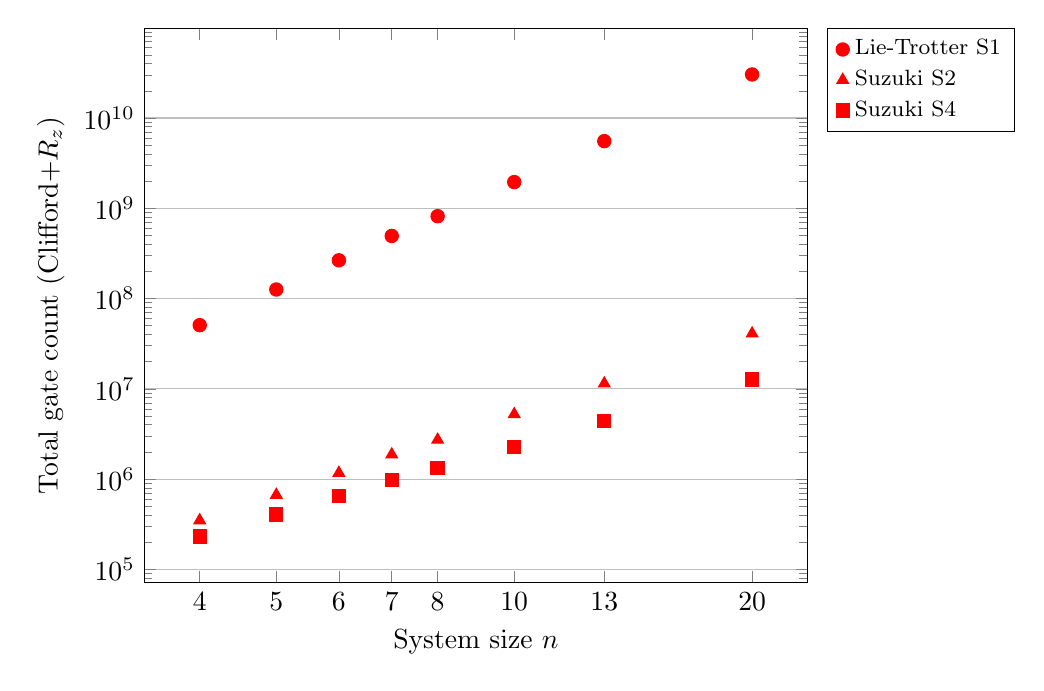
\begin{tikzpicture}
  \begin{loglogaxis}[
    width=10cm,
    xlabel={System size $n$},
    ylabel={Total gate count (Clifford+$R_z$)},
    xtick={4,5,6,7,8,10,13,20},
    xticklabels={4,5,6,7,8,10,13,20},
    ymajorgrids=true,
    legend pos=outer north east,
    legend cell align=left,
    legend style={font=\footnotesize},
  ]
    \addplot[only marks, red, mark=*, mark size=2.4pt, mark options={solid, fill=red}] coordinates {
      (4,50712168)
      (5,126015370)
      (6,265272852)
      (7,493871560)
      (8,817749296)
      (10,1951302340)
      (13,5545632586)
      (20,30391954320)
    };
    \addlegendentry{Lie-Trotter S1}
    \addplot[only marks, red, mark=triangle*, mark size=2.4pt, mark options={solid, fill=red}] coordinates {
      (4,348864)
      (5,667440)
      (6,1168992)
      (7,1870512)
      (8,2721792)
      (10,5222400)
      (13,11443536)
      (20,40893120)
    };
    \addlegendentry{Suzuki S2}
    \addplot[only marks, red, mark=square*, mark size=2.4pt, mark options={solid, fill=red}] coordinates {
      (4,230656)
      (5,403860)
      (6,644904)
      (7,976472)
      (8,1322880)
      (10,2283240)
      (13,4404088)
      (20,12664880)
    };
    \addlegendentry{Suzuki S4}
  \end{loglogaxis}
\end{tikzpicture}
